\documentclass[10pt,letterpaper]{article}
\usepackage{toolsper}
\settextfont{B Nazanin}
\usepackage{lipsum}
\begin{document}
\Large
\begin{center}
به نام خدا

تمرینات سری اول درس شبکه‌های مخابراتی

مهلت تحویل : 16 مهرماه 98
\hl
\end{center}
\noindent
سوال 1) درستی یا نادرستی گزاره های زیر را با بیان دلایل کافی تحقیق کنید.

1. برای شدت ترافیک نزدیک به $1$، تاخیر صف
\footnote{
\lr{Queuing delay}
}
 بسته ها به سمت صفر میل می کند.

2. داده برای انتقال از یک هاست
\footnote{
\lr{Host}
}
 به هاست دیگر، فقط از مجموعه ای از لینک ها می گذرد.

3. \lr{API} 
مجموعه‌ی قوانینی است که برنامه‌ی سمت فرستنده باید پیروی کند تا اینترنت قادر به انتقال داده به برنامه‌ی مقصد باشد.

4. \lr{Packet Switching}
 پیاده سازی پیچیده تر و پر هزینه تری نسبت به \lr{Circuit Switching} ایجاب می کند؛ ولی در مقابل برای کاربردهای بلادرنگ
\footnote{
\lr{Real-time}
}
 مناسب تر است.

5. یک پروتکل، فرمت و ترتیب پیامهای جابجاشده بین دو واحد مخابراتی را مشخص می کند و به اعمال انجام شده در ارسال و یا دریافت پیام نظارتی ندارد.

6. در سمت کاربر، \lr{DSLAM} وظیفه ی جداسازی سیگنال های تلفنی و دیتای اینترنتی را در \lr{cable Internet access} بر عهده دارد.

7. در معماری \lr{PON} همه ی بسته های ارسال شده از \lr{OLT} به سمت \lr{Splitter}، در \lr{Splitter} تکثیر می شوند.

8. به دلایل اقتصادی، از فیبر نوری نمی توان در شبکه های \lr{long-haul} استفاده کرد.

9. لایه‌ی پروتکل فقط در نرم افزار پیاده سازی می‌شود.

10. تنها یک پروتکل \lr{IP} وجود دارد و تمام اجزای اینترنت که یک لایه‌ی شبکه دارند، باید از این پروتکل تبعیت کنند.

\noindent
سوال 2) تفاوت ویروس (\lr{Virus}) و کرم (\lr{Worm}) چیست؟

\noindent
 سوال 3) در یک روتر، بسته
\footnote{
\lr{Packet}
}
 هایی با طول 8 بیت به ورودی آن ارسال می شوند و نرخ دریافت بسته ها در ورودی از توزیع زیر پیروی می کند:
\eqn{
f_A(a)={(3.35)^a\cdot e^{-3.35}\over a!}
}{}
نرخ خروجی بیت در روتر نیز دارای توزیع زیر است:
\eqn{
R\sim \mathcal{U}(35,40)
}{}
\indent
الف) متوسط شدت ترافیک
\footnote{
\lr{Traffic Intensity}
}
 را در این روتر محاسبه کنید.

\indent
ب) اگر چهار بسته به صورت پشت سر هم وارد این روتر شوند، متوسط تاخیر ارسال
\footnote{
\lr{Transmission delay}
}
 بسته‌ی چهارم چه 
\indent
میزان خواهد بود؟ (تاخیر ارسال بسته‌ی اول را صفر در نظر بگیرید)

\noindent
سوال 4) در شبکه ی زیر، اگر احتمال خرابی هر لینک مستقل از سایرین برابر $p$ باشد، احتمال صحت کل مسیر را از $A$ تا $B$ به دست آورید.
\begin{center}
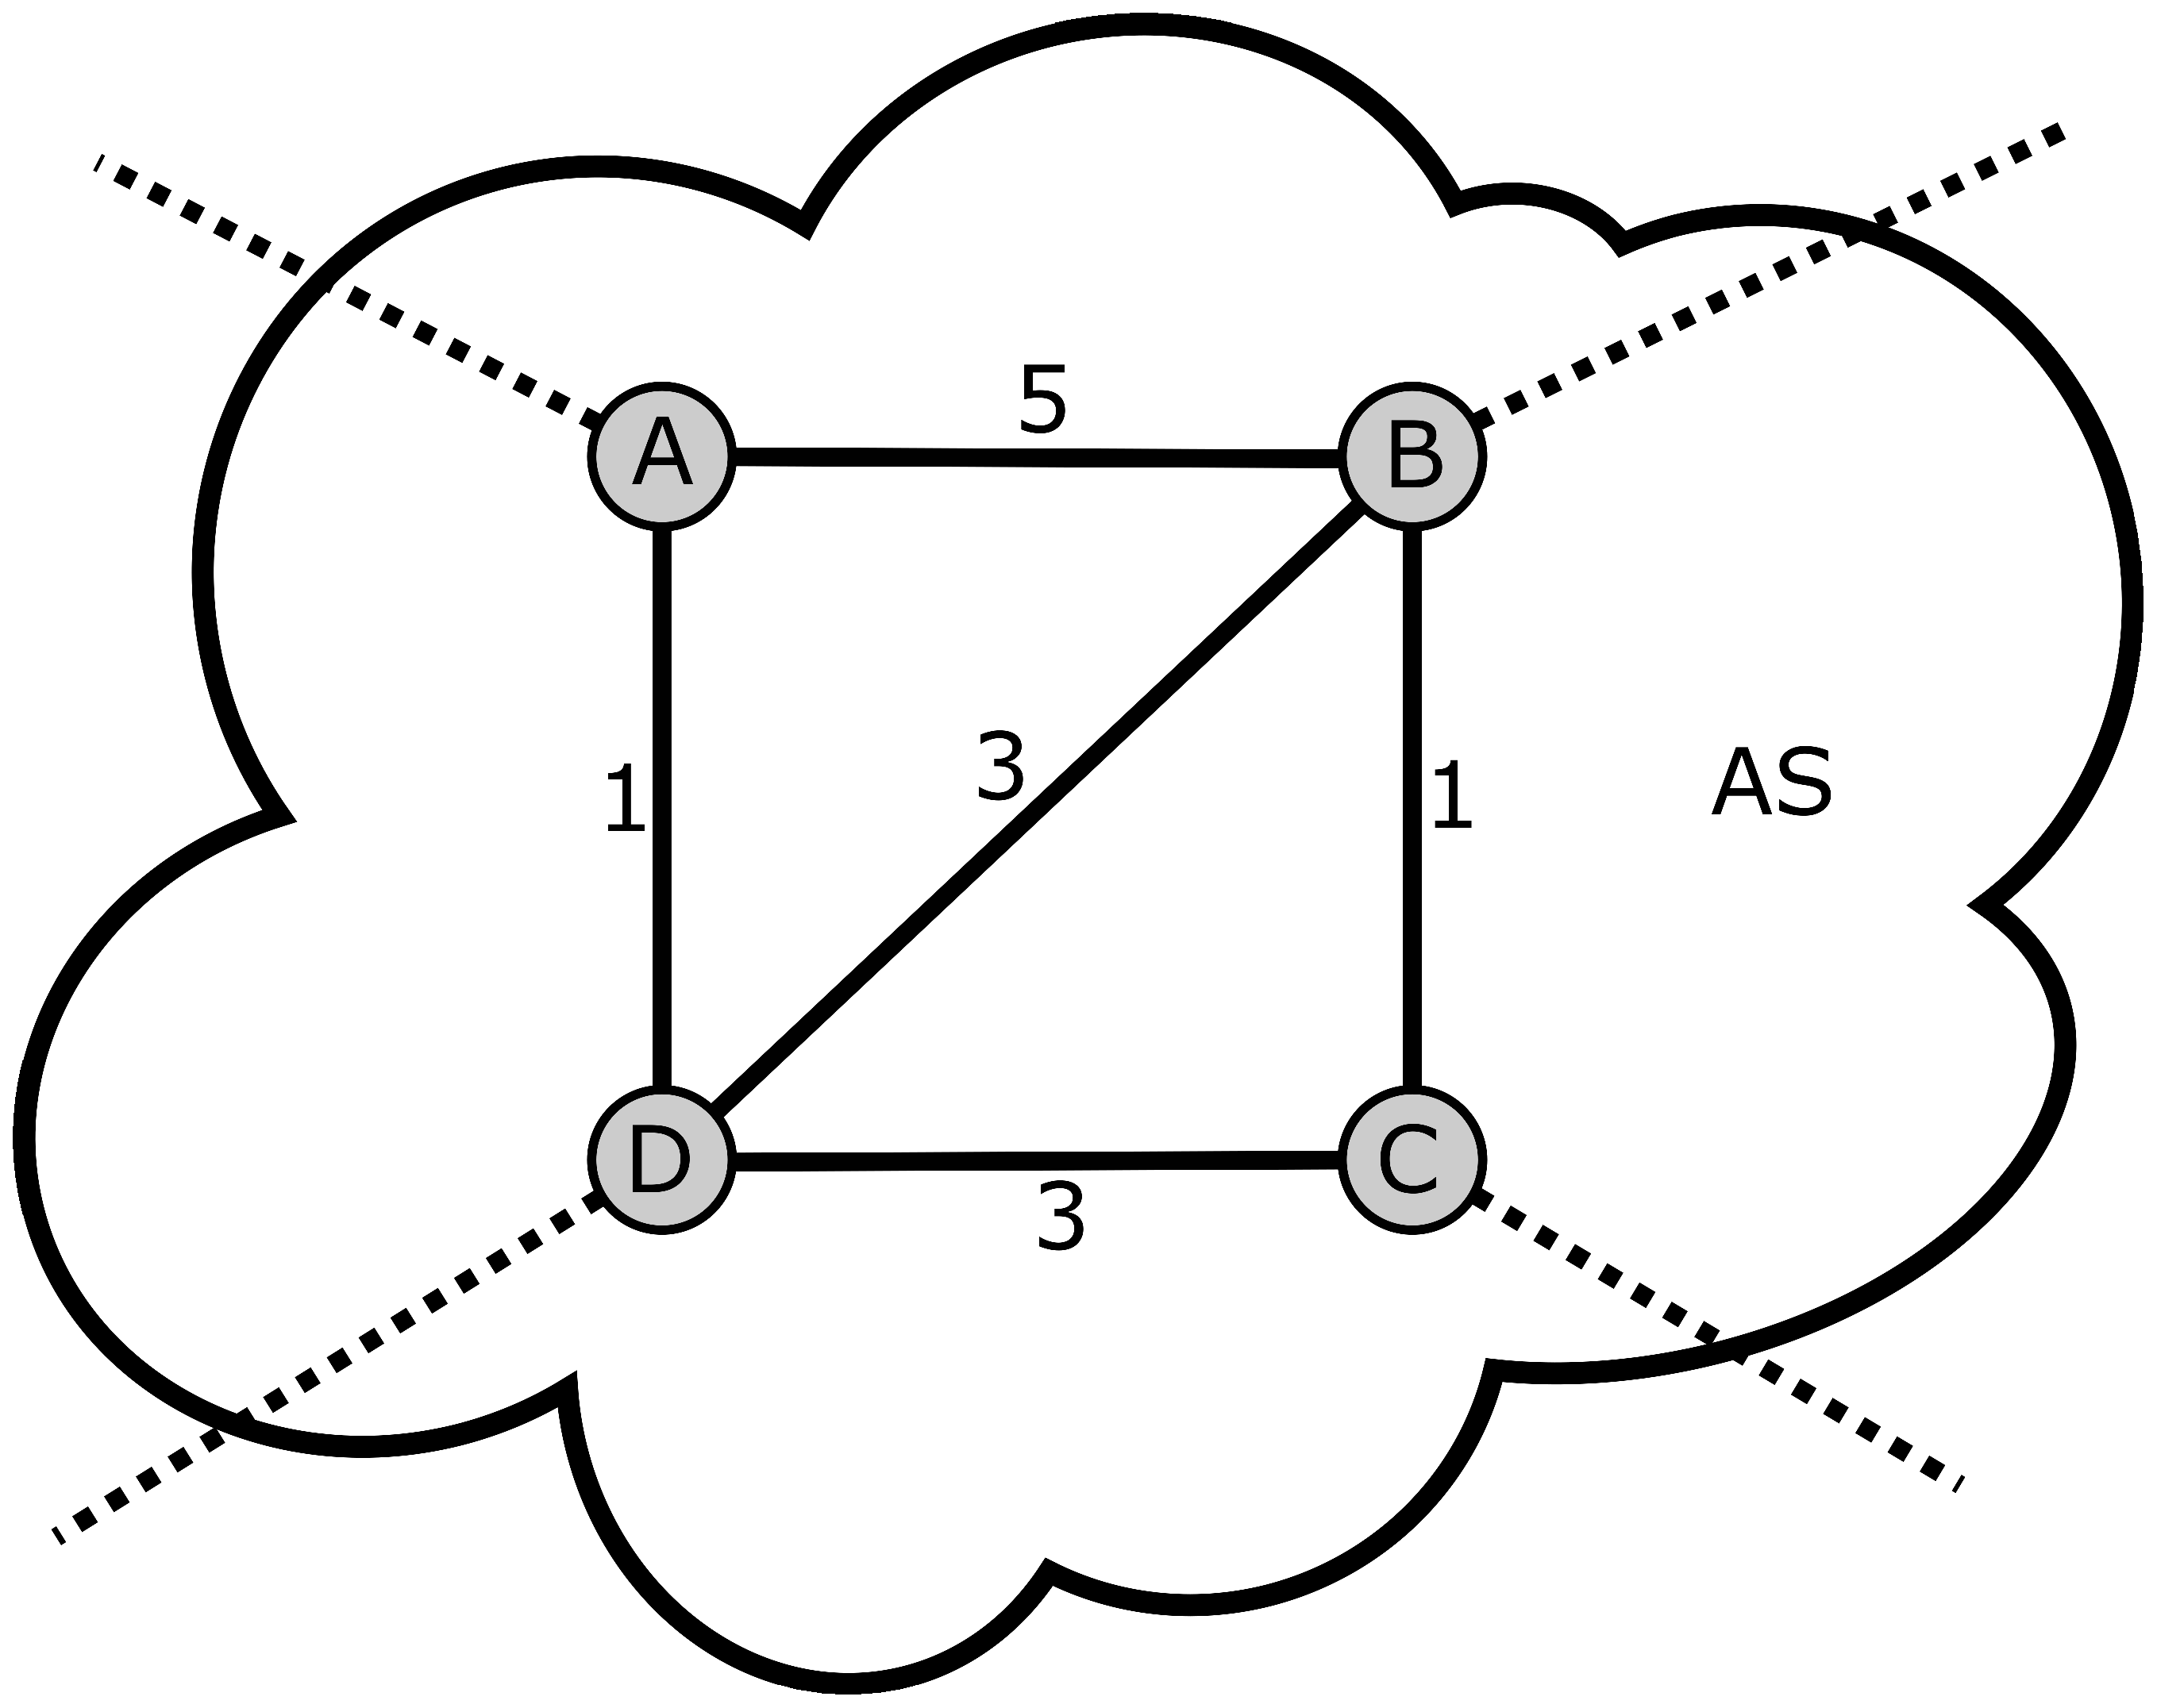
\includegraphics[width=100mm]{Q4}
\end{center}
سوال 5) در شبکه ای با توپولوژی زیر، در چه صورت و با کدام احتمال حداکثر \lr{throughput} برای مسیر $A-H$ برابر $2R$ می باشد؟ (احتمال خرابی هر لینک مستقل از سایرین برابر $p$ می باشد)
\begin{center}
\includegraphics[width=100mm]{Q5}
\end{center}
\noindent
سوال 6) در شبکه‌ی زیر، فرض کنید نرخ ورود بیت به روتر برابر 
$1\text{\lr{Mbps}}$
، حجم هر بسته برابر 
$1\text{\lr{kbytes}}$
، تاخیر پردازش هر بسته برابر 
$12\text{\lr{msec}}$
، طول لینک برابر 200 متر و سرعت انتشار در لینک برابر 
$2\times 10^8 \text{\lr{m/s}}$
 است. همچنین  نرخ خروج بیت از روتر را بینهایت بگیرید.

الف) تاخیر ارسال را برای بسته‌ی دهم محاسبه کنید.

ب) تاخیر کلی ای را که بسته‌ی دوم در ارسال از \lr{A} به \lr{B} تجربه می کند محاسبه کنید.

ج) به مدت چند میلی ثانیه و برای اولین بار، حجم اشغال شده‌ی بافر برابر 
$2\text{\lr{kbytes}}$
 خواهد بود؟ (حالتی که یک بسته بلافاصله وارد بافر می‌شود و تنها بسته‌ی کنونی بافر بلافاصله از آن خارج می‌شود، $1\text{\lr{kbytes}}$ از حجم بافر را اشغال می‌کند. به عبارت دیگر باید مدت زمان غیرصفری محاسبه شود که دو بسته همزمان در بافر حضور داشته باشند)
\begin{center}
\includegraphics[width=100mm]{Q6.jpg}
\end{center}
\end{document}